% Created 2021-02-24 mié 12:40
% Intended LaTeX compiler: pdflatex
\documentclass[presentation,aspectratio=169]{beamer}
\usepackage[utf8]{inputenc}
\usepackage[T1]{fontenc}
\usepackage{graphicx}
\usepackage{grffile}
\usepackage{longtable}
\usepackage{wrapfig}
\usepackage{rotating}
\usepackage[normalem]{ulem}
\usepackage{amsmath}
\usepackage{textcomp}
\usepackage{amssymb}
\usepackage{capt-of}
\usepackage{hyperref}
\usepackage{khpreamble}
\usepackage{amssymb}
\usepgfplotslibrary{groupplots}
\usepackage{gensymb}
\newcommand*{\shift}{\operatorname{q}}
\usetheme{default}
\author{Kjartan Halvorsen}
\date{2021-02-15}
\title{Sensores, Encoder incremental}
\hypersetup{
 pdfauthor={Kjartan Halvorsen},
 pdftitle={Sensores, Encoder incremental},
 pdfkeywords={},
 pdfsubject={},
 pdfcreator={Emacs 26.3 (Org mode 9.4.4)}, 
 pdflang={English}}
\begin{document}

\maketitle

\section{Sensores en general}
\label{sec:orgf890ffa}
\begin{frame}[label={sec:org04797ee}]{Sensores}
\begin{center}
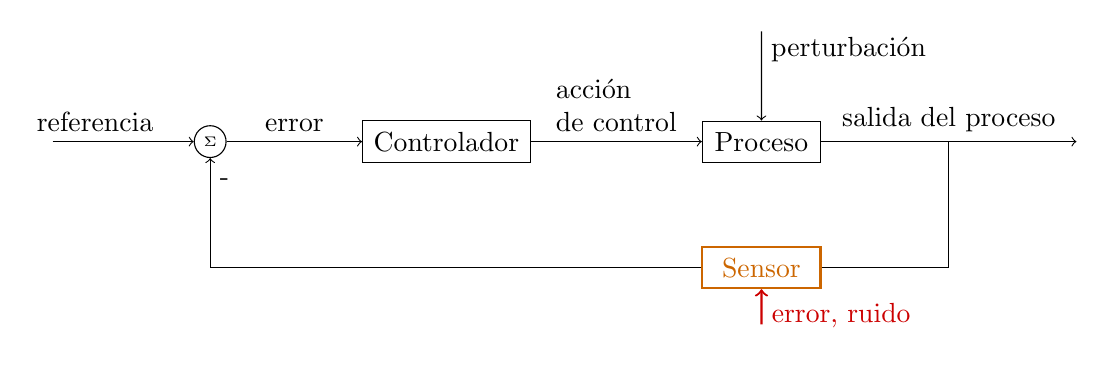
\begin{tikzpicture}[scale=0.6, node distance=22mm, block/.style={rectangle, draw, minimum width=15mm, inner sep=4pt}, sumnode/.style={circle, draw, inner sep=2pt}]

  \node[coordinate] (input) {};
  \node[sumnode, right of=input, node distance=20mm] (sumerr) {\tiny $\Sigma$};
  \node[block, right of=sumerr, node distance=30mm] (fb)  {Controlador};
  \node[block, right of=fb, node distance=40mm] (plant)  {Proceso};
  \node[block, orange!80!black, thick, below of=plant, node distance=16mm] (sensor)  {Sensor};

  \node[coordinate, above of=plant, node distance=14mm] (disturbance) {};
  \node[coordinate, right of=plant, node distance=40mm] (output) {};

  \draw[->] (input) -- node[above, pos=0.3] {referencia} (sumerr);
  \draw[->] (sumerr) -- node[above] {error} (fb);
  \draw[->] (fb) -- node[above, align=left,] {acción \\de control} (plant);
  \draw[->] (plant) -- node[coordinate] (meas) {} node[above,] {salida del proceso} (output);
  \draw[->] (disturbance) -- node[right, pos=0.2] {perturbación} (plant);
  \draw[->] (meas) |- (sensor) -| node[right, pos=0.9] {-} (sumerr);
  \draw[->, red!80!black, thick] (sensor) ++(0, -12mm) -- node[near start, right] {error, ruido} (sensor);
  \end{tikzpicture}
\end{center}

Es \alert{inevitable} que el uso de sensores introduzca \alert{ruido} en el sistema.
\end{frame}

\begin{frame}[label={sec:orgcb27a5e}]{Sensores}
\begin{center}
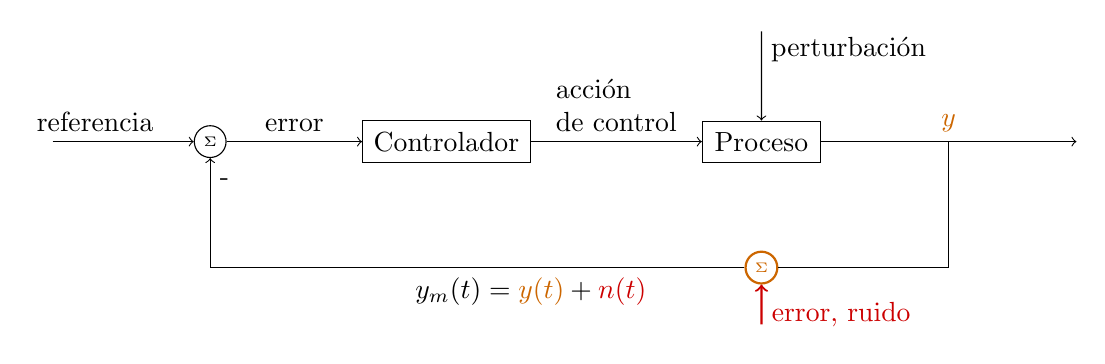
\begin{tikzpicture}[scale=0.6, node distance=22mm, block/.style={rectangle, draw, minimum width=15mm, inner sep=4pt}, sumnode/.style={circle, draw, inner sep=2pt}]

  \node[coordinate] (input) {};
  \node[sumnode, right of=input, node distance=20mm] (sumerr) {\tiny $\Sigma$};
  \node[block, right of=sumerr, node distance=30mm] (fb)  {Controlador};
  \node[block, right of=fb, node distance=40mm] (plant)  {Proceso};
  \node[sumnode, orange!80!black, thick, below of=plant, node distance=16mm] (sensor)  {\tiny $\Sigma$};


  \node[coordinate, above of=plant, node distance=14mm] (disturbance) {};
  \node[coordinate, right of=plant, node distance=40mm] (output) {};

  \draw[->] (input) -- node[above, pos=0.3] {referencia} (sumerr);
  \draw[->] (sumerr) -- node[above] {error} (fb);
  \draw[->] (fb) -- node[above, align=left,] {acción \\de control} (plant);
  \draw[->] (plant) -- node[coordinate] (meas) {} node[above, orange!80!black] {$y$} (output);
  \draw[->] (disturbance) -- node[right, pos=0.2] {perturbación} (plant);
  \draw[->] (meas) |- (sensor) -| node[pos = 0.2, below] {$y_m(t) = \textcolor{orange!80!black}{y(t)} + \textcolor{red!80!black}{n(t)}$} node[right, pos=0.9] {-} (sumerr);
  \draw[->, red!80!black, thick] (sensor) ++(0, -12mm) -- node[near start, right] {error, ruido} (sensor);
  \end{tikzpicture}
\end{center}

Es \alert{importante} conocer las caracteristicas (estadisticas) del error de medida!

\begin{center}
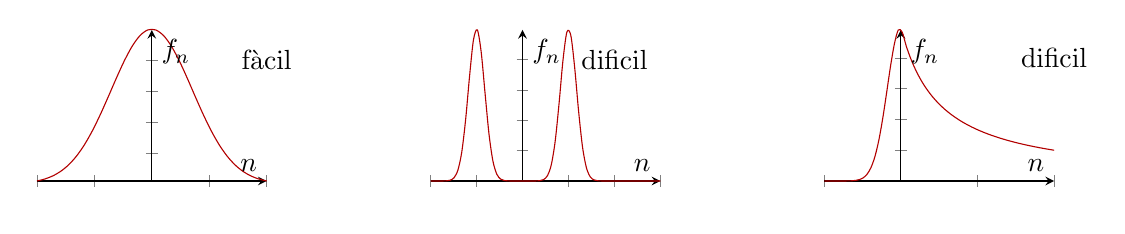
\begin{tikzpicture}
  \begin{axis}[clip=false,width=4.5cm, height=3.5cm, xticklabel=\empty, yticklabel=\empty,
  axis lines=middle,
  ylabel={$f_n$}, xlabel={$n$}]
  \addplot[red!70!black, no marks, smooth, domain=-2:2, samples=30] {exp(-pow(x,2))};
  \node at (axis cs: 2,0.8) {fàcil};
  \end{axis}
  \begin{axis}[clip=false, xshift=5cm, width=4.5cm, height=3.5cm, xticklabel=\empty, yticklabel=\empty,
  axis lines=middle,
  ylabel={$f_n$}, xlabel={$n$}]
  \addplot[red!70!black, no marks, smooth, domain=-4:6, samples=60] {exp(-pow((x-2)*2,2)) + exp(-pow((x+2)*2,2)) };
  \node at (axis cs: 4,0.8) {dificil};
  \end{axis}
  \begin{axis}[clip=false, xshift=10cm, width=4.5cm, height=3.5cm, xticklabel=\empty, yticklabel=\empty,
  axis lines=middle,
  ylabel={$f_n$}, xlabel={$n$}]
  \addplot[red!70!black, no marks, smooth, domain=-2:4, samples=60] {(x<0)*exp(-pow((x)*2,2)) + (x>=0)/(1+x) };
  \node at (axis cs: 4,0.8) {dificil};
  \end{axis}
\end{tikzpicture}
\end{center}
\end{frame}


\begin{frame}[label={sec:org2b97254}]{Sensores - características}
\begin{itemize}
\item \alert{Exactitud} Que tán correcto es en promedio.  \alert{Precisón} Desviación del error.
\item \alert{Sensibildad o resolución} El cambio más pequeño en la señal que se puede detectar.
\item \alert{Retraso} \(y_m(t) = y(t-\tau) + n(t)\)
\item \alert{Muestreo y digitalización}
\begin{center}
\includegraphics[width=0.8\textwidth]{../../figures/sampling-digitalization}
\end{center}
\end{itemize}
\end{frame}

\section{Encoder}
\label{sec:org6940255}
\begin{frame}[label={sec:org00a43d0}]{Encoder incremental}
\begin{center}
\includegraphics[width=0.7\textwidth]{../../figures/encoder-im.jpg}
{\footnotesize Fuente: \url{https://www.sciencedirect.com/topics/engineering/incremental-encoder}}
\end{center}
\end{frame}

\begin{frame}[label={sec:org7cff6cb}]{Encoder incremental}
\begin{center}
\includegraphics[width=0.4\textwidth]{../../figures/encoder-disc}
\includegraphics[width=0.5\textwidth]{../../figures/encoder-signals}
\end{center}

\emph{Pulses Per Revolution (PPR)} es igual a 4 en el ejemplo. Cada apertura tiene un sector de \(\frac{360\degrees}{2 \times PPR} = 45\degree\).
\end{frame}

\begin{frame}[label={sec:org13f283c}]{Encoder incremental}
\begin{center}
\includegraphics[width=0.4\textwidth]{../../figures/encoder-disc}
\includegraphics[width=0.5\textwidth]{../../figures/encoder-signals}
\end{center}

\alert{Actividad individual} Si detectamos los flancos positivos \alert{y} los flancos negativos de las dos señales \textcolor{blue!80!black}{A} y \textcolor{red!80!black}{B}. Cual sería el giro minimo que podemos detectar (la sensitivad del sensor)?
\end{frame}


\begin{frame}[label={sec:orgabca622}]{Encoder incremental}
\begin{center}
\includegraphics[width=0.4\textwidth]{../../figures/encoder-disc}
\includegraphics[width=0.5\textwidth]{../../figures/encoder-signals}
\end{center}

\alert{Actividad individual} En el ejemplo arriba, el encoder gira en sentido del reloj (CW) o en sentido contrario al reloj (CCW)?
\end{frame}


\begin{frame}[label={sec:org329bda1}]{Encoder incremental - Velocidad}
\begin{columns}
\begin{column}{0.5\columnwidth}
\begin{center}
\includegraphics[width=\textwidth]{../../figures/encoder-signals-nonuniform}
\end{center}
\end{column}
\begin{column}{0.5\columnwidth}
Se requiere la velocidad angular del eje en el instante \(t=\unit{6.5}{\milli\second}\). El número de pulsos por revolución es PPR=8, y contamos cada flanco (ascendente y descendente) de cada señal A y B, que resulte en 32 conteos por revolución.

\alert{Actividad individual} Computa la velocidad angular en rad/s en los casos \alert{(a)} usando un tiempo de rastreo de \(\Delta t=\unit{0.5}{\milli\second}\), \alert{(b)} usando un tiempo de rastreo \(\Delta t=\unit{5}{\milli\second}\).
\end{column}
\end{columns}
\end{frame}






\begin{frame}[label={sec:org5e6269f}]{Encoder incremental - Velocidad por frequencia}
\begin{columns}
\begin{column}{0.5\columnwidth}
\begin{center}
\includegraphics[width=\textwidth]{../../figures/encoder-signals-freqs}
\end{center}
\end{column}
\begin{column}{0.5\columnwidth}
La velocidad tambien se puede medir usando el tiempo entre pulsos. En el ejemplo hubo un intervalo de \unit{1}{\milli\second} entre los dos pulsos. Este da la velocidad
\begin{align*}
 v &= 1 \, \text{pulsos/ms} = \frac{1/32 \, \text{revoluciones}}{\unit{10^{-3}}{\second}}\\
 &= \unit{\frac{2\pi}{32}\times 1000}{\rad\per\second} = \unit{196.3}{\rad\per\second}
 \end{align*}
\end{column}
\end{columns}
\end{frame}






\begin{frame}[label={sec:org36b2be8}]{Encoder incremental - Velocidad por frequencia}
\begin{columns}
\begin{column}{0.5\columnwidth}
\begin{center}
\includegraphics[width=\textwidth]{../../figures/encoder-signals-nonuniform}
\end{center}
\end{column}
\begin{column}{0.5\columnwidth}
\alert{Actividad individual} Calcula la velocidad!
\end{column}
\end{columns}
\end{frame}






\begin{frame}[label={sec:org7d9020f}]{Encoder incremental - Velocidad por frequencia}
\begin{columns}
\begin{column}{0.7\columnwidth}
\begin{center}
\includegraphics[width=0.8\textwidth]{../../figures/encoder-signal-freqs2}
\end{center}
\end{column}

\begin{column}{0.3\columnwidth}
La velocidad solo se calcula cuando viene un pulso.
\end{column}
\end{columns}
\end{frame}
\end{document}